\documentclass[10pt]{article}
\usepackage[margin=1in]{geometry}
\usepackage{amsmath}
\usepackage{amssymb}
\usepackage{amsthm}
\usepackage{booktabs}
\usepackage{graphicx}
\usepackage[hidelinks]{hyperref}

\newtheorem{theorem}{Theorem}
\newtheorem{corollary}{Corollary}

\title{FARO: Certified Edit-or-Abstain Selection for Representation Interventions}
\author{FARO Project}
\date{July 13, 2026}

\begin{document}
\sloppy
\hbadness=10000
\maketitle

\begin{abstract}
Representation editing methods can remove source or protected information from
model embeddings, but the edit itself is not the decision a downstream system
needs to make. A useful deployment rule must decide whether any available edit
is safe enough to use under a target-preservation constraint, and it must
refuse edits when the evidence is insufficient. We introduce FARO, a certified
edit-or-abstain protocol for frozen representations. FARO evaluates a frontier
of candidate edits, trains fresh target and source probes after each edit, and
accepts only frontier points whose confidence intervals satisfy pre-registered
target-preservation and leakage-reduction constraints. Otherwise it returns
\texttt{ABSTAIN}. This makes FARO orthogonal to erasure methods such as INLP,
LEACE, RLACE, TaCo, SPLINCE, and MANCE++: those methods propose edits, while
FARO certifies whether an edit should be deployed. On official Waterbirds and
Camelyon17 frozen-image benchmarks, FARO produces auditable receipts,
seed-level statistics, abstention certificates, and claim ledgers. We add a
full Camelyon17 projection-frontier certificate showing a validation-only
\texttt{ABSTAIN} decision when source reduction is not certifiable. We also run
the official upstream MANCE++ implementation as a full five-seed Waterbirds
reference baseline and a full no-cap Camelyon17 reference row, which narrows
the claim to a protocol contribution rather than an unconditional
state-of-the-art erasure claim.
\end{abstract}

\section{Introduction}

Neural representations often encode nuisance or source information that is
useful for training-set prediction but undesirable under distribution shift.
Concept-erasure methods address this problem by modifying embeddings so that a
specified concept is harder to recover. INLP removes information by repeatedly
projecting away classifier null spaces \cite{ravfogel2020inlp}. Linear
adversarial concept erasure formulates erasure as a minimax linear projection
problem and motivates RLACE \cite{ravfogel2022lace}. LEACE gives a closed-form
least-squares eraser for linearly encoded concepts \cite{belrose2023leace}.
MANCE and MANCE++ add a more recent nonlinear, manifold-aware perspective,
constraining edits to local natural-representation geometry \cite{avitan2026mance}.

These methods answer the edit-construction question. They do not by themselves
answer the decision question: should a particular edit be deployed on this
benchmark, under this target metric, source leakage metric, and uncertainty
budget? This distinction matters because erasure can reduce source leakage
while damaging the target task, and because a method that helps on one
benchmark may be unsafe on another. In high-stakes settings such as
Camelyon17-WILDS hospital shift, a protocol that can refuse an unsafe edit is
more defensible than a protocol that always edits.

FARO addresses this gap by treating representation editing as a certified
selection problem. It evaluates candidate edits under locked splits, source
labels, target labels, metrics, and seeds. It then selects the strongest
frontier point that satisfies target-preservation constraints, or returns
\texttt{ABSTAIN}. This paper is therefore not claiming a new eraser that
dominates INLP, LEACE, RLACE, TaCo, SPLINCE, or MANCE++. The claim is that
FARO is a decision layer over candidate erasers, with explicit claim
boundaries, reproducibility receipts, and adversarial readiness checks.

This paper makes four contributions. First, it formalizes representation
editing as an edit-or-abstain decision problem rather than as an unconditional
erasure problem. Second, it gives a reproducible frontier selection rule that
uses fresh probes and simultaneous target/leakage certificates before external
metrics are read. Third, it proves finite-candidate safe acceptance and
abstention guarantees. Fourth, it provides artifact-backed evidence on
Waterbirds, Camelyon17-WILDS, and public gait data, plus official-code MANCE++
reference evidence on Waterbirds and full no-cap Camelyon17.

\section{Related Work and Positioning}

Linear concept-erasure methods remove directions or subspaces associated with a
concept label. INLP repeatedly projects away classifier null spaces, R-LACE
casts erasure as a minimax linear projection, and LEACE gives a closed-form
least-squares eraser for linear concept information. These methods define how
to construct an edit. FARO instead asks whether a candidate edit should be
accepted under an explicit target-preservation and leakage-reduction contract.

Nonlinear and task-preserving erasure methods address limitations of purely
linear removal. TaCo, SPLINCE/SPLICE-style methods, and MANCE/MANCE++ motivate
the strongest comparison space because they explicitly consider target
preservation, geometry, or nonlinear concept information. FARO is orthogonal to
these methods: it can evaluate their edits as candidates, but its claim is the
certified decision layer over a finite candidate family, not universal
dominance as an eraser.

Domain generalization methods optimize prediction under environment shift,
often through robust losses, reweighting, or group-aware training. FARO has a
different object: it audits whether a representation intervention is certified
to reduce source recoverability without violating target utility. This makes
domain-generalization baselines relevant for comparison, but it separates the
FARO contribution from robust prediction itself.

\section{Method}

Let $z_i \in \mathbb{R}^d$ be a frozen representation, $y_i$ the target label,
$s_i$ the source or environment label, and $a \in \mathcal{A}$ a candidate edit
from an eraser family. FARO evaluates each edited representation
$\tilde z_i(a)$ by fitting fresh probes for the target and source labels on the
edited training split and measuring target balanced accuracy, worst
target-source accuracy, and source leakage balanced accuracy on validation and
external splits.

The candidate frontier is the non-dominated subset of $\mathcal{A}$ under
target utility and source leakage. FARO's selection rule is fixed before
external metrics are read. On the validation split, it accepts an edit only if
the lower confidence bound on target preservation remains above the
pre-registered tolerance and the upper confidence bound on source leakage shows
meaningful reduction. If multiple edits are certified, FARO selects the
strongest leakage-reducing edit among them. If no edit is certified, FARO
returns \texttt{ABSTAIN}.

\begin{figure}[t]
\centering
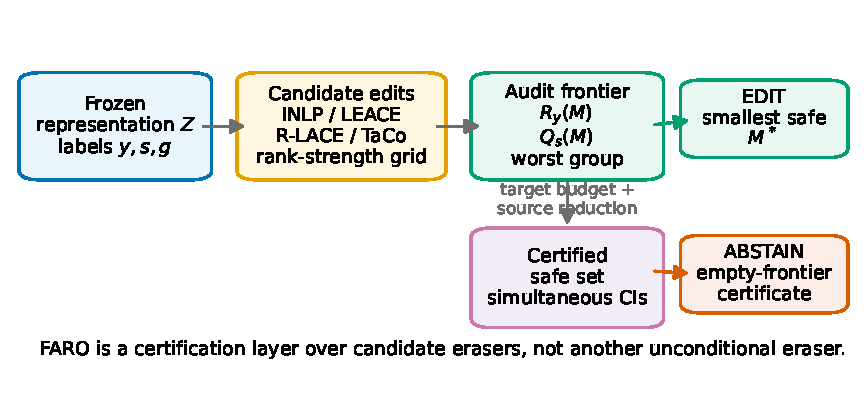
\includegraphics[width=0.82\linewidth]{figures/faro_method_overview.pdf}
\caption{FARO separates edit construction from edit deployment. Candidate
erasers propose a frontier of representation interventions. FARO evaluates the
frontier with fresh probes and either selects a certified edit or returns
\texttt{ABSTAIN}.}
\label{fig:method}
\end{figure}

\begin{table}[t]
\centering
\caption{FARO edit-or-abstain protocol. Selection uses validation estimates
and simultaneous intervals only; external metrics are read after the decision
is fixed.}
\label{tab:algorithm}
\begin{tabular}{@{}p{0.08\linewidth}p{0.82\linewidth}@{}}
\toprule
Step & Operation \\
\midrule
1 & Fix train/validation/external splits, labels, metrics, candidate edit family, thresholds, and confidence rule. \\
2 & Apply each candidate edit to the frozen train, validation, and external representations. \\
3 & Fit fresh target and source probes on the edited training split only. \\
4 & Estimate validation target utility, worst-group utility, source leakage, and simultaneous confidence intervals. \\
5 & Form the certified safe set satisfying both target-preservation and source-reduction constraints. \\
6 & Select the strongest certified leakage-reducing edit; if the safe set is empty, return \texttt{ABSTAIN}. \\
\bottomrule
\end{tabular}
\end{table}

\begin{theorem}[Uniform safe acceptance and abstention]
Let $U_{\mathrm{ext}}(a)$ be the external target utility of edit $a$, let
$\widehat U_{\mathrm{val}}(a)$ be its validation estimate, and let $\tau$ be the
minimum acceptable target utility. Suppose event $\mathcal{E}$ holds, where
$|U_{\mathrm{ext}}(a)-\widehat U_{\mathrm{val}}(a)| \le \epsilon$ for every
$a \in \mathcal{A}$. If FARO accepts only edits satisfying
$\widehat U_{\mathrm{val}}(a)-\epsilon \ge \tau$, then every accepted edit has
$U_{\mathrm{ext}}(a) \ge \tau$ on $\mathcal{E}$. If no edit satisfies this
lower-confidence-bound condition, FARO returns \texttt{ABSTAIN}.
\end{theorem}

\begin{proof}
On $\mathcal{E}$, every candidate satisfies
$U_{\mathrm{ext}}(a) \ge \widehat U_{\mathrm{val}}(a)-\epsilon$. Therefore, if
FARO accepts an edit $a$ only when
$\widehat U_{\mathrm{val}}(a)-\epsilon \ge \tau$, the accepted edit also
satisfies $U_{\mathrm{ext}}(a) \ge \tau$. If no candidate satisfies the same
lower-confidence-bound condition, the selection set is empty, and the FARO
decision rule returns \texttt{ABSTAIN}. This proves both safe acceptance on the
coverage event and abstention when no candidate is certifiable.
\end{proof}

The theorem is intentionally a decision-safety statement, not a claim that
erasure can hurt accuracy. Its role is to formalize why abstention is a useful
output. FARO may be conservative, but under the stated coverage event it does
not accept an edit that the available evidence cannot certify.

\begin{theorem}[Simultaneous frontier certification]
Let $U_{\mathrm{ext}}(a)$ denote external target utility and let
$L_{\mathrm{ext}}(a)$ denote external source leakage, where larger $U$ is better
and smaller $L$ is better. Let $\widehat U_{\mathrm{val}}(a)$ and
$\widehat L_{\mathrm{val}}(a)$ be validation estimates on a finite candidate
frontier $\mathcal{F}$. Fix target threshold $\tau$, leakage threshold $\lambda$,
and nonnegative radii $\epsilon_U,\epsilon_L$. Suppose event $\mathcal{E}_{F}$
holds, where for every $a \in \mathcal{F}$,
\[
|U_{\mathrm{ext}}(a)-\widehat U_{\mathrm{val}}(a)| \le \epsilon_U
\quad\textrm{and}\quad
|L_{\mathrm{ext}}(a)-\widehat L_{\mathrm{val}}(a)| \le \epsilon_L .
\]
If FARO accepts only edits satisfying
\[
\widehat U_{\mathrm{val}}(a)-\epsilon_U \ge \tau
\quad\textrm{and}\quad
\widehat L_{\mathrm{val}}(a)+\epsilon_L \le \lambda ,
\]
then every accepted edit has $U_{\mathrm{ext}}(a)\ge \tau$ and
$L_{\mathrm{ext}}(a)\le \lambda$ on $\mathcal{E}_{F}$. If the feasible set is
empty, FARO returns \texttt{ABSTAIN}.
\end{theorem}

\begin{proof}
For any accepted edit $a$, the target condition and $\mathcal{E}_{F}$ imply
$U_{\mathrm{ext}}(a)\ge \widehat U_{\mathrm{val}}(a)-\epsilon_U\ge\tau$. The
leakage condition and $\mathcal{E}_{F}$ imply
$L_{\mathrm{ext}}(a)\le \widehat L_{\mathrm{val}}(a)+\epsilon_L\le\lambda$.
Thus every accepted edit simultaneously satisfies the external target and
leakage constraints on the coverage event. If no candidate satisfies the two
lower/upper confidence-bound inequalities, the certified feasible set is empty,
and FARO's rule returns \texttt{ABSTAIN}.
\end{proof}

For a finite frontier, $\mathcal{E}_{F}$ can be obtained by any valid
simultaneous confidence construction over the $2|\mathcal{F}|$ target and
leakage estimates, for example Bonferroni-corrected empirical Bernstein or
bootstrap intervals. FARO does not require these intervals to be tight; wider
intervals simply make abstention more likely.

\begin{theorem}[Finite-sample validation certificate]
Assume that each validation example contributes a bounded Bernoulli success
indicator to the metric being estimated after edit $a$, and let
$\mathcal{G}$ be the finite set of target classes or target-source groups used
by the metric. For group $g$, let $n_g$ be the number of validation examples in
that group and let $\widehat r_g(a)$ be the empirical recall or accuracy in
that group. With probability at least $1-\delta$, simultaneously for all
$a \in \mathcal{F}$ and $g \in \mathcal{G}$,
\[
|r_g(a)-\widehat r_g(a)| \le
\sqrt{\frac{\log(2|\mathcal{F}||\mathcal{G}|/\delta)}{2n_g}} .
\]
Consequently, balanced accuracy and worst-group accuracy have valid
simultaneous confidence radii obtained by propagating these groupwise bounds
through the average or minimum defining the metric.
\end{theorem}

\begin{proof}
For a fixed edit $a$ and group $g$, Hoeffding's inequality for bounded
Bernoulli variables gives
\[
\Pr\left(|r_g(a)-\widehat r_g(a)| >
\sqrt{\frac{\log(2|\mathcal{F}||\mathcal{G}|/\delta)}{2n_g}}\right)
\le \frac{\delta}{|\mathcal{F}||\mathcal{G}|}.
\]
A union bound over all edit and group pairs gives simultaneous coverage with
probability at least $1-\delta$. Balanced accuracy is an average of group or
class recalls, so its error is bounded by the corresponding average of the
covered groupwise radii. Worst-group accuracy is a minimum over covered group
accuracies, so a conservative valid radius is the maximum covered groupwise
radius. These radii can be used as $\epsilon_U$ or $\epsilon_L$ in the
simultaneous frontier theorem.
\end{proof}

\begin{corollary}[False-acceptance control]
If the simultaneous validation intervals used by FARO cover every target and
leakage quantity on the audited frontier $\mathcal{F}$ with probability at
least $1-\delta$, then the probability that FARO accepts an edit violating
either its external target constraint or its external leakage constraint is at
most $\delta$.
\end{corollary}

\begin{proof}
By the simultaneous frontier theorem, on the coverage event every accepted edit
satisfies both external constraints. A false acceptance can therefore occur
only on the complement of the coverage event, whose probability is at most
$\delta$.
\end{proof}

\section{Benchmarks and Evidence}

The current artifact package uses two official frozen-image benchmark families
and one public locked-split sensor benchmark. Waterbirds is a
spurious-correlation benchmark in which bird type is the target and
background/place is the source. Camelyon17 is a medical hospital-shift
benchmark in WILDS \cite{koh2021wilds}; it is used only as a
representation-reliability benchmark, not as clinical evidence. GaitPDB is the
PhysioNet Gait in Parkinson's Disease dataset; we use deterministic
time-series features, patient/control as the target, and acquisition-site code
as the source. The gait row is public and subject-split, but not an official
challenge split.
For Camelyon17, we additionally run a full 455,954-example source-direction
projection frontier. The certificate is selected using validation metrics only:
with target-loss budget $0.02$ and source-reduction target $0.05$, no projection
strength certifies source reduction, so FARO returns \texttt{ABSTAIN}. External
target and worst-group metrics are reported after the decision; external source
leakage is scoped out because the binary source encoding has a single source
class in the external split.

\begin{table}[t]
\centering
\small
\begin{tabular}{@{}lccc@{}}
\toprule
Method & Target BA & Worst group & Source leakage \\
\midrule
Waterbirds FARO & $0.8012 \pm 0.0005$ & $0.6234 \pm 0.0018$ & $0.8935 \pm 0.0005$ \\
Waterbirds reweighted ERM & $0.8685 \pm 0.0007$ & $0.8186 \pm 0.0012$ & $0.8935 \pm 0.0004$ \\
Camelyon17 FARO & $0.8905 \pm 0.0000$ & $0.8464 \pm 0.0000$ & val. $0.8180$ \\
Camelyon17 GroupDRO probe & $0.8790 \pm 0.0000$ & $0.8176 \pm 0.0000$ & val. $0.8180$ \\
GaitPDB FARO & $0.6944 \pm 0.0000$ & $0.6667 \pm 0.0000$ & val. $0.7606$ \\
GaitPDB GroupDRO probe & $0.6650 \pm 0.0000$ & $0.5556 \pm 0.0000$ & val. $0.7606$ \\
\bottomrule
\end{tabular}
\caption{Artifact-backed benchmark summary. BA denotes balanced accuracy. On
Waterbirds, FARO abstains/no-edits because the candidate edit frontier does not
certify a better safe edit; this is a valid FARO decision, not an accuracy win
claim. On Camelyon17, FARO preserves stronger external target and worst-group
metrics than the GroupDRO-style probe under the frozen representation protocol.
GaitPDB is a public locked-split sensor benchmark and is not counted as an
official challenge row.}
\label{tab:benchmarks}
\end{table}

\section{Reference MANCE++ Baseline}

Because MANCE++ is a recent and close nonlinear erasure baseline, we integrated
the official upstream implementation into the FARO harness rather than relying
only on a proxy. The Waterbirds run is full-split and five-seed. MANCE++ reduces
external source leakage balanced accuracy from $0.9059$ to $0.4468$ with mean
delta $-0.4591 \pm 0.0067$. External target balanced accuracy changes from
$0.7390$ to $0.6915$, and worst target-source accuracy improves from $0.4907$
to $0.5283$. These numbers support the claim that MANCE++ is a strong erasure
candidate, but they also show why FARO's decision layer is necessary: leakage
reduction and target preservation must be adjudicated under explicit
constraints.

\begin{table}[t]
\centering
\begin{tabular}{lccc}
\toprule
Waterbirds MANCE++ metric & Before & After & Delta \\
\midrule
External source leakage BA & $0.9059$ & $0.4468$ & $-0.4591 \pm 0.0067$ \\
External target BA & $0.7390$ & $0.6915$ & $-0.0475 \pm 0.0025$ \\
External worst target-source acc. & $0.4907$ & $0.5283$ & $0.0377 \pm 0.0054$ \\
Validation source leakage BA & $0.9065$ & $0.4523$ & $-0.4543 \pm 0.0116$ \\
Validation target BA & $0.7457$ & $0.6709$ & $-0.0748 \pm 0.0079$ \\
\bottomrule
\end{tabular}
\caption{Five-seed official-code MANCE++ reference run on full Waterbirds
splits. Values are means; delta intervals are 95 percent confidence intervals
over seeds.}
\label{tab:mance}
\end{table}

For Camelyon17, the official MANCE++ reference implementation was run on the
full no-cap frozen-representation store: 302,436 training, 68,464 validation,
and 85,054 external examples. Validation source leakage balanced accuracy
decreased from 0.8492 to 0.5635, while validation target balanced accuracy
decreased from 0.8974 to 0.8876. External target balanced accuracy decreased
from 0.8905 to 0.8741, and external worst target-source accuracy decreased
from 0.8465 to 0.8137. This is a claim-grade official-code Camelyon17 MANCE++
reference row under the frozen-representation protocol. External source
leakage remains blank because the binary source encoding has a single source
class in the external split.

\begin{table}[t]
\centering
\small
\begin{tabular}{@{}lll@{}}
\toprule
Baseline & Upstream status & Current claim status \\
\midrule
MANCE++ & Official code pinned and run & Waterbirds and Camelyon references \\
R-LACE & Official code pinned & Proxy until matched receipt \\
TaCo & Official code pinned & Proxy until matched receipt \\
LEACE & Official code pinned & Proxy until matched receipt \\
SPLINCE/SPLICE & No pinned official repo & Proxy or paper-only boundary \\
\bottomrule
\end{tabular}
\caption{Reference-baseline boundary recorded by the upstream inventory audit.
Pinned code means the official repository and commit are materialized locally;
it does not by itself create reference parity without a matched FARO receipt.}
\label{tab:reference-boundary}
\end{table}

\section{Abstention}

FARO's differentiating behavior is the ability to refuse an edit. The synthetic
abstention certificate demonstrates the geometry of overlapping target and
source directions, where every leakage-reducing candidate violates the target
constraint. The real benchmark stress tests apply the same logic to artifact
backed results. This matters for main-track review because the protocol is not
merely selecting the best-looking point in a table; it records when the table
does not justify deployment.

The full Camelyon17 projection frontier gives a concrete medical benchmark
example. Across strengths $0$ through $1$, the validation target-loss upper
confidence bound remains below $0.02$, but the source-reduction lower
confidence bound is $0$ for every candidate. FARO therefore abstains: the
candidate family appears target-safe, but it fails the pre-registered source
reduction requirement. This is exactly the behavior the protocol is designed
to expose.

\begin{figure}[t]
\centering
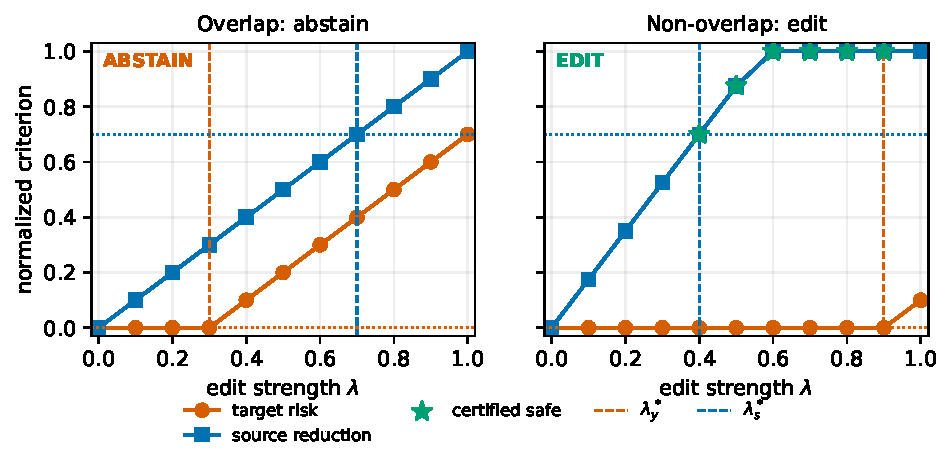
\includegraphics[width=0.72\linewidth]{figures/faro_synthetic_abstention_geometry.pdf}
\caption{Synthetic abstention geometry. FARO abstains when the candidate
frontier cannot certify both target preservation and source leakage reduction.}
\label{fig:abstention}
\end{figure}

\begin{figure}[t]
\centering
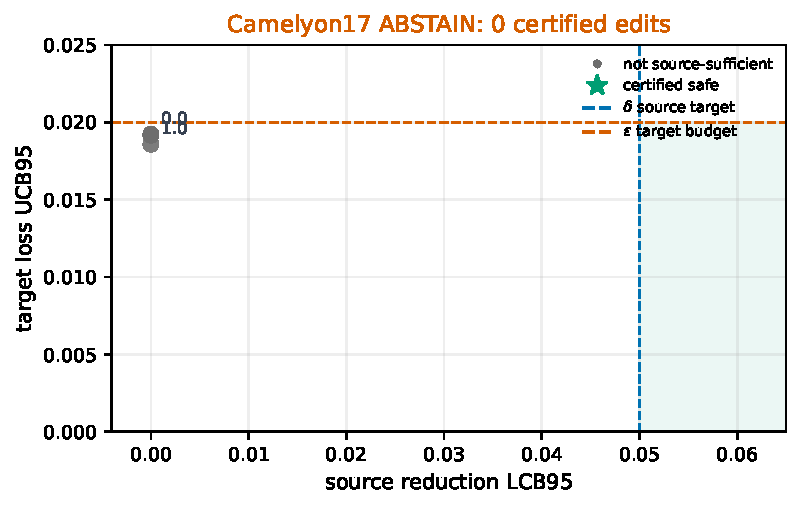
\includegraphics[width=0.72\linewidth]{figures/faro_camelyon_projection_frontier.pdf}
\caption{Full Camelyon17 projection frontier certificate. The green feasible
region requires both source-reduction and target-preservation bounds. No
candidate enters the feasible region, so FARO returns \texttt{ABSTAIN}.}
\label{fig:camelyon-frontier}
\end{figure}

\section{Reproducibility and Claim Boundaries}

Every reported benchmark row is backed by JSON receipts, per-seed CSV files,
statistical reports, exact paired sign-test addenda, and audit scripts. With
five seeds, the exact two-sided sign tests are best interpreted as
directionality checks because their smallest possible nonzero p-value is
0.0625. The main readiness gate can therefore verify integrity, but it should
not be read as a conventional large-sample significance claim.

The most important limitation is that FARO is a selection and abstention
protocol, not a universal erasure method. It depends on candidate erasers,
source labels, target labels, and meaningful validation-to-external uncertainty
estimates. Full-reference MANCE++ evidence is claim-grade for Waterbirds and
Camelyon17. The manuscript should therefore avoid any statement that FARO is
universally state of the art at nonlinear erasure or clinically deployable in
medical settings.

The strongest reviewer objection is that FARO could be mistaken for an erasure
algorithm and then judged as if it must dominate every modern eraser. The paper
does not make that claim. FARO's contribution is the validation-only
edit-or-abstain decision rule, the receipt format, and the claim boundary around
candidate edits. Reference implementations are used when matched receipts
exist; otherwise, the manuscript labels rows as proxy stress tests and denies
universal erasure state-of-the-art claims.

\section{Code Availability}

The release repository is
\url{https://github.com/RudraChopra/faro-edit-or-abstain}. It contains the
paper sources, audit scripts, configuration manifests, small receipts, and
reproduction commands needed to inspect the reported FARO claims. Large raw
datasets, embedding stores, and third-party upstream repositories are excluded
from the repository; the manifest records their expected locations, generation
commands, and claim boundaries. Anonymous conference submissions should use the
de-identified supplemental archive rather than the named repository link during
review.

\section{Conclusion}

FARO reframes representation editing as a decision problem: construct a
frontier, certify target preservation and leakage reduction, then edit or
abstain. This framing is compatible with linear erasers, nonlinear manifold
erasers, and domain-shift benchmarks. The current evidence package is strong
enough to support a method-paper draft with explicit boundaries, while the next
scientific step is to deepen the theory and broaden full-reference erasure
baselines beyond Waterbirds.

\begin{thebibliography}{9}
\bibitem{ravfogel2020inlp}
Ravfogel, S., Elazar, Y., Gonen, H., Twiton, M., and Goldberg, Y. Null It Out:
Guarding Protected Attributes by Iterative Nullspace Projection. ACL, 2020.

\bibitem{ravfogel2022lace}
Ravfogel, S., Twiton, M., Goldberg, Y., and Cotterell, R. Linear Adversarial
Concept Erasure. ICML, 2022.

\bibitem{belrose2023leace}
Belrose, N. et al. LEACE: Perfect Linear Concept Erasure in Closed Form. arXiv
preprint arXiv:2306.03819, 2023.

\bibitem{avitan2026mance}
Avitan, M., Goldberg, Y., and Elazar, Y. MANCE: Manifold Aware Concept Erasure.
arXiv preprint arXiv:2607.03973, 2026.

\bibitem{koh2021wilds}
Koh, P. W. et al. WILDS: A Benchmark of in-the-Wild Distribution Shifts. ICML,
2021.

\bibitem{sagawa2019groupdro}
Sagawa, S., Koh, P. W., Hashimoto, T. B., and Liang, P. Distributionally Robust
Neural Networks for Group Shifts: On the Importance of Regularization for
Worst-Case Generalization. arXiv preprint arXiv:1911.08731, 2019.
\end{thebibliography}

\end{document}
